\section{Results and Analysis}
\subsection{Geometry: low error does not imply completeness}
\begin{table}[t]
\centering\small
\begin{tabular}{lrrr}
\toprule
Subset / region & Coverage & Bad$>1$ & RMSE (m)\\
\midrule
13 eval / all & 61.26\% & 46.38\% & 0.1201\\
13 eval / nonocc. & 67.14\% & 39.87\% & 0.1016\\
15 incl.\ dev / all & 62.65\% & 44.73\% & 0.1498\\
\bottomrule
\end{tabular}
\caption{StereoSGBM. Coverage and Bad$>1$ are pixel-pooled; Bad includes invalid output. RMSE is a scene-average conditional depth error. The 15-scene row includes development data.}
\label{tab:stereo}
\end{table}
Table~\ref{tab:stereo} exposes the coverage cost of correspondence filtering. On the 13 evaluation scenes, 38.74\% of all-GT pixels have no valid prediction despite a conditional RMSE of 0.1201 m. Restricting to officially nonoccluded GT improves coverage to 67.14\%, but considerable failure remains. Thus occlusion alone cannot explain all missing output.

\begin{figure*}[t]
\centering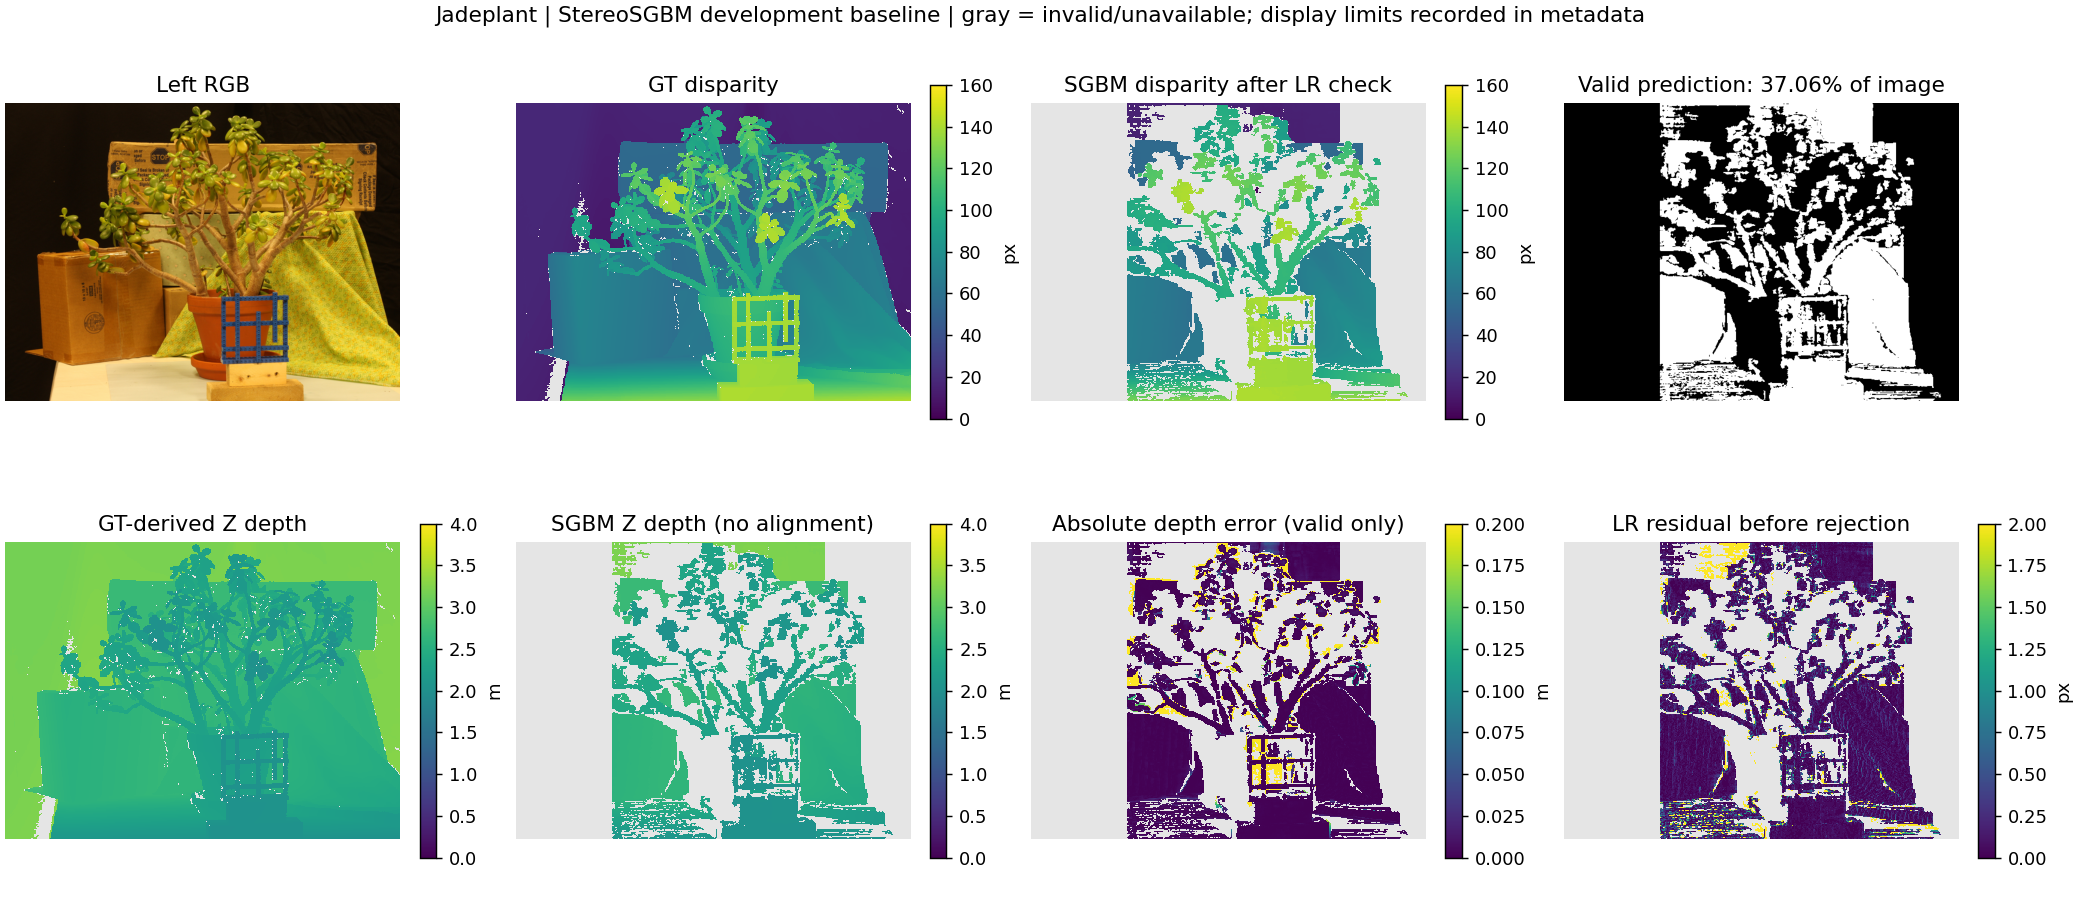
\includegraphics[width=\textwidth]{images/stereo_jadeplant.png}
\caption{Jadeplant StereoSGBM diagnostics. Gray means invalid/unavailable. Thin leaves, branches, and the foreground grid contain substantial missing predictions. The mask-panel percentage uses the entire image as denominator; metric coverage uses the fixed valid-GT region. Saturated colors are display limits, not prediction clipping.}
\label{fig:stereo}
\end{figure*}
Figure~\ref{fig:stereo} shows Jadeplant, where all-GT coverage is 37.39\% and conditional RMSE is 0.1291 m. Gaps concentrate around leaves, thin branches, and the foreground structure. Correspondence ambiguity, occlusion, and windows crossing depth boundaries are plausible explanations, but were not isolated by causal ablation. PianoL has 39.42\% coverage and 0.3594 m RMSE, including incorrect surviving wall matches. A small left--right residual is therefore insufficient to prove correctness. Pipes, a development scene, reaches 0.5913 m RMSE; Eq.~\ref{eq:stereo} explains depth sensitivity to disparity errors, but visual saturation alone cannot measure the error.

\subsection{NYUv2: direct metric and aligned relative depth}
\begin{table*}[t]
\centering\small
\begin{tabular}{lrrrrrrrr}
\toprule
Model / evaluation & AbsRel & SqRel & RMSE & RMSE-log & $\delta_1$ & $\delta_2$ & $\delta_3$ & Coverage\\
\midrule
UniDepthV2 ViT-S / metric & .11224 & .08299 & .41666 & .14001 & .89311 & .97906 & .99265 & 100\%\\
DA V2-S Hypersim / metric & .28011 & .29076 & .81515 & .26115 & .51993 & .91384 & .98476 & 100\%\\
\midrule
DA V2-S relative / GT aligned & .06210 & .04464 & .31135 & .09388 & .95525 & .98786 & .99595 & 99.8471\%\\
\bottomrule
\end{tabular}
\caption{NYUv2 standard 654-image split. SqRel and RMSE use metres; RMSE-log uses natural logarithms. The seven metrics are conditional image averages. The relative row uses GT and has 653 contributing images, one alignment failure, and full-GT $\delta_{1/2/3}=.95379/.98635/.99442$. It is not ranked as a direct metric model. Both direct models contribute all 654 images.}
\label{tab:nyu}
\end{table*}
Table~\ref{tab:nyu} reports all required depth metrics. Under the recorded matched-resolution configuration, UniDepthV2 outperforms the DA Hypersim metric checkpoint in AbsRel, RMSE, and all three threshold scores. Both predict valid values over the complete GT region, so this difference does not arise from dropping more pixels. The comparison does not establish a ranking across other model sizes, training distributions, or resolutions.

The relative model has lower conditional errors after fitting two parameters to every image's GT inverse depth. This measures aligned structure, not equally informed metric inference. Image \texttt{nyuv2\_0650} produces a fitted slope of approximately $-0.04944$, violating the declared inverse-depth direction. We retain this failure and its original array. Silently excluding it would change both the population and the meaning of the score.

\begin{table}[t]
\centering\small
\begin{tabular}{lrrrr}
\toprule
Model & Precision & Recall & F1 & Dist.\ (px)\\
\midrule
UniDepthV2 & .7551 & .3999 & .5229 & 5.324\\
DA metric & .6680 & .4068 & .5057 & 5.185\\
DA rel.\ aligned & .6698 & .5045 & .5755 & 4.174\\
\bottomrule
\end{tabular}
\caption{Depth-discontinuity results, with 2,295,868 GT edge pixels shared by all models. The relative row includes GT alignment and its failed case. Distance is GT-to-prediction, capped at 10 pixels.}
\label{tab:edges}
\end{table}
Table~\ref{tab:edges} reveals a more nuanced boundary comparison. UniDepth has higher precision than DA metric, but slightly lower recall and larger capped GT-to-prediction distance. Its F1 advantage does not mean it recovers every boundary more completely. Absolute-scale error and discontinuity localization remain distinct measurements.

\begin{figure*}[t]
\centering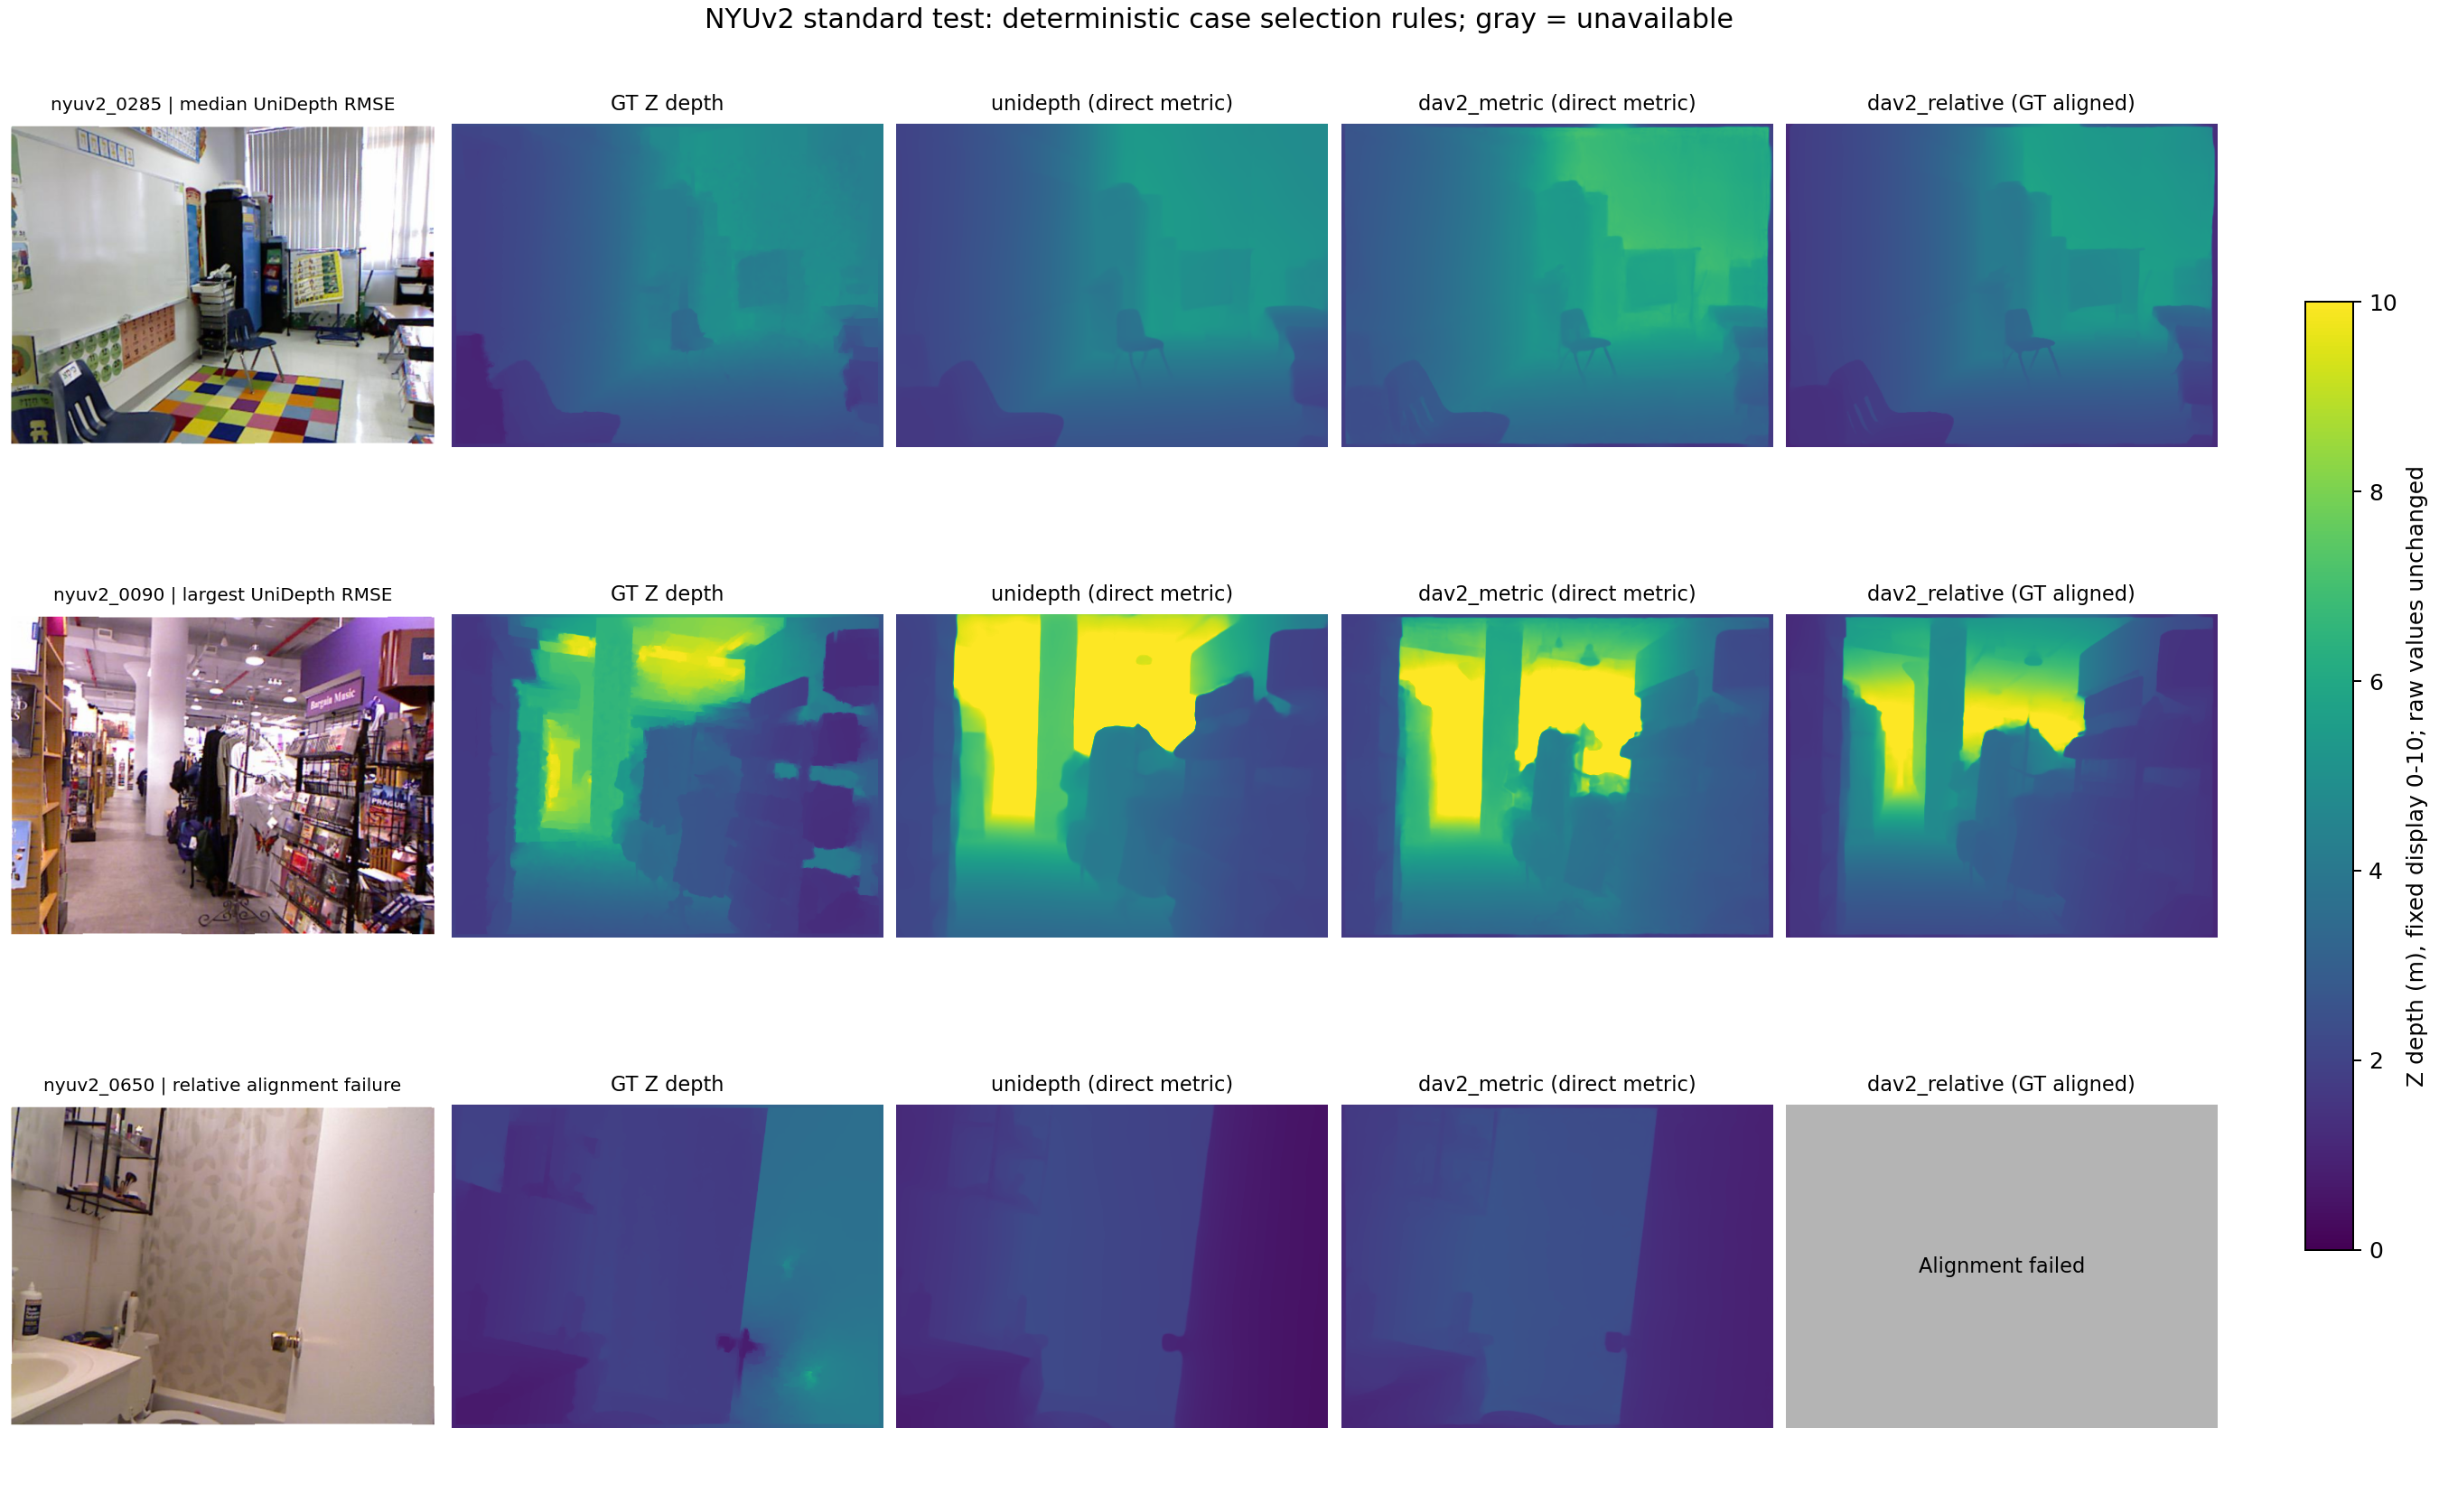
\includegraphics[width=\textwidth]{images/nyu_comparison.png}
\caption{Deterministically selected NYUv2 cases: UniDepth median-RMSE image 0285, maximum-RMSE image 0090, and relative-alignment failure 0650. All depth panels use 0--10 m; gray denotes missing aligned output. The relative column uses GT, whereas direct metric columns do not.}
\label{fig:nyu}
\end{figure*}


The examples in Figure~\ref{fig:nyu} follow recorded selection rules. UniDepth's maximum-error sample has RMSE 3.9283 m: a good dataset mean does not exclude large individual errors. The alignment-failure image contains a mirror. Reflection may disrupt the relation between apparent content and measured depth, but this image alone does not establish the cause. Final video analysis still needs independent glass, sky, blur, and thin-structure cases.

\subsection{Compute cost}
\begin{table*}[t]
\centering\small
\begin{tabular}{lrrrrrr}
\toprule
Model & Params (M) & Weight (MB) & Time (ms) & FPS & Alloc.\ (GiB) & Reserved (GiB)\\
\midrule
UniDepthV2 ViT-S & 34.184 & 136.778 & 43.68 & 22.89 & .393 & .445\\
DA V2-S metric & 24.785 & 99.222 & 56.83 & 17.60 & .270 & .311\\
DA V2-S relative & 24.785 & 99.218 & 58.53 & 17.08 & .270 & .311\\
\bottomrule
\end{tabular}
\caption{One complete NYUv2 run per model, FP16 with actual encoder input $434\times574$ and output $480\times640$. MB is decimal; GiB is binary. Timing excludes I/O/evaluation. No repeated-run confidence interval is claimed.}
\label{tab:cost}
\end{table*}
Table~\ref{tab:cost} reports measured inference cost. Parameter count alone does not predict this pipeline's latency, which also includes model-specific preprocessing and restoration. The stated timing boundaries permit comparison without claiming an isolated kernel benchmark.

Before recording development footage, VDA resource tests on the same 24-frame public example used short sides 280, 364, and 518, producing actual inputs $280\times504$, $364\times644$, and $518\times924$. Peak allocated memory was 1.089, 2.309, and 7.807 GiB, with throughput 20.22, 9.06, and 0.92 fps. At 518, allocator-reserved memory reached 11.58 GiB; we cannot infer that all of it occupied dedicated VRAM or attribute the slowdown to a measured shared-memory mechanism. We selected 364 as a resource setting before self-recorded experiments. A padded 24-frame clip is not a long-video performance estimate.

\subsection{Temporal implementation evidence}
The example has 23 adjacent pairs and 1,293,996 shared reference pixels. Recomputing saved RGB flows, masks, E0--E4 arrays, fusion weights, and all E0--E5 scores reproduced the stored values. Conditional temporal L1 on this example is 0.2800 m for E0, 0.1088 for EMA, and 0.2026 for E4. These are program checks, not final test outcomes or parameter-selection evidence. EMA's lower value may reflect delayed response rather than better geometry. Cross-model absolute differences are also influenced by their different scales.

Analytical tests cover known image translation, warp direction, invalid interpolation, consistency rejection, and true depth change. They verify that motion alignment avoids the same-pixel EMA ghost in the controlled translation case and that adaptive weights reduce history influence when depth changes. Such tests establish mechanics, not real-world effectiveness.

Formal E0--E5 conclusions remain pending. Development will inspect static fluctuation, thin-boundary retention, approach/retreat response, and occlusion recovery alongside the fixed-denominator scores. After freezing a small configuration, the same analysis will run on independent test clips. If no candidate provides a useful trade-off, that negative result will be retained rather than replaced by the best example score.

